\documentclass[]{beamer}
\usepackage[T1]{fontenc}
\usepackage[utf8]{inputenc}
\usepackage{lmodern}
\usepackage[italian]{babel}

\title{Account Google}
\author{Mattia Cozzi}
\date{a.f.~2024/2025}


%\documentclass[handout]{beamer}     %usare questa classe per generare l'handout

%\usepackage{pdfpages}   %per mostrare più quadri nella stessa pagina
%\pgfpagesuselayout{4 on 1}[a4paper,border shrink=5mm,landscape]


\usetheme{Singapore}
%\useoutertheme[left]{sidebar} %elementi intorno alle diapositive
\setbeamercovered{dynamic} %modifica l'aspetto del testo grigetto delle diapositive future. Argomenti: invisible/transparent/dynamic


%COLORE PRINCIPALE
\definecolor{verde}{RGB}{2, 194, 117} % UBC Blue (primary)
\setbeamercolor{structure}{fg=verde} % itemize, enumerate, etc
\setbeamercolor{alerted text}{fg=verde}


\usecolortheme{orchid}

\usepackage{tikz}

\begin{document}

\begin{frame}
  \titlepage
\end{frame}


\begin{frame}
\frametitle{Contenuti}
\tableofcontents
\end{frame}



\section{Account}


\begin{frame}
\frametitle{Cosa è un account}
Un account è una \alert{registrazione presso un servizio}, come un conto in banca.\pause

~

Quando abbiamo un conto in banca, possiamo entrare in banca, essere riconosciuti e fare operazioni con i nostri dati o il nostro denaro.

\visible<2->{\begin{figure}
  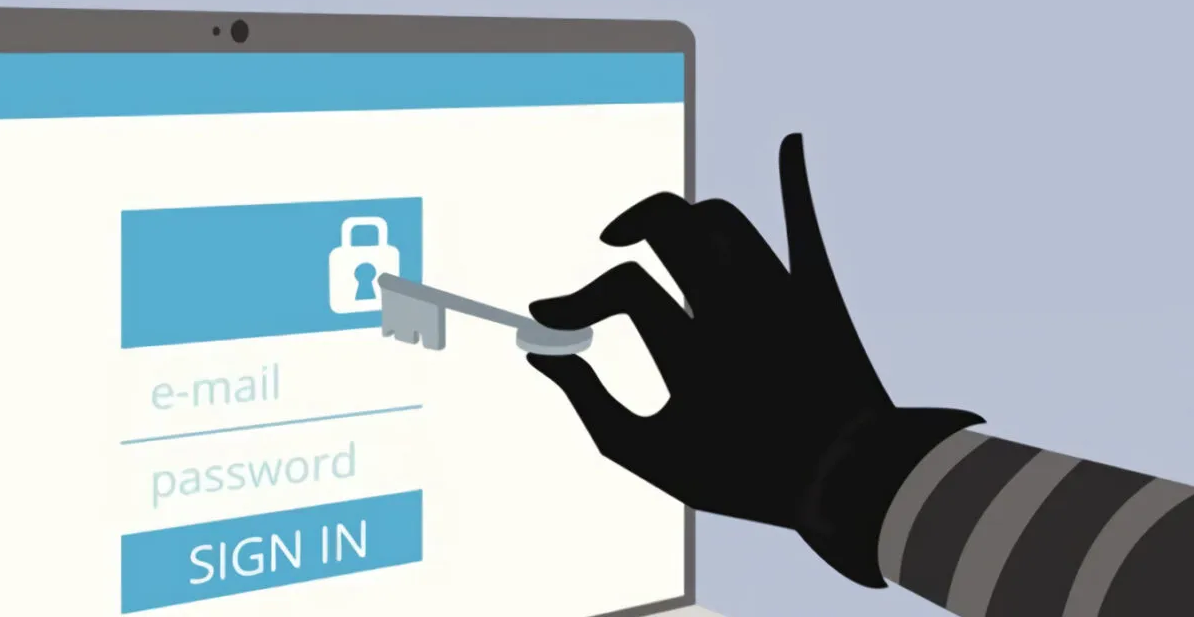
\includegraphics[width=.6\columnwidth]{img/account.png}
\end{figure}}
\end{frame}




\begin{frame}
\frametitle{Accesso (login) ad un account}
Per confermare la nostra identità, dobbiamo \alert{accedere al nostro account} presso un servizio.\pause

~

L'accesso, detto comunemente \alert{login}, richiede un \alert{nome utente (username)} e una \alert{password}.

A volte è richiesta l'autenticazione in due passaggi (ad esempio con un messaggio sul cellulare).

\visible<2->{\begin{figure}
  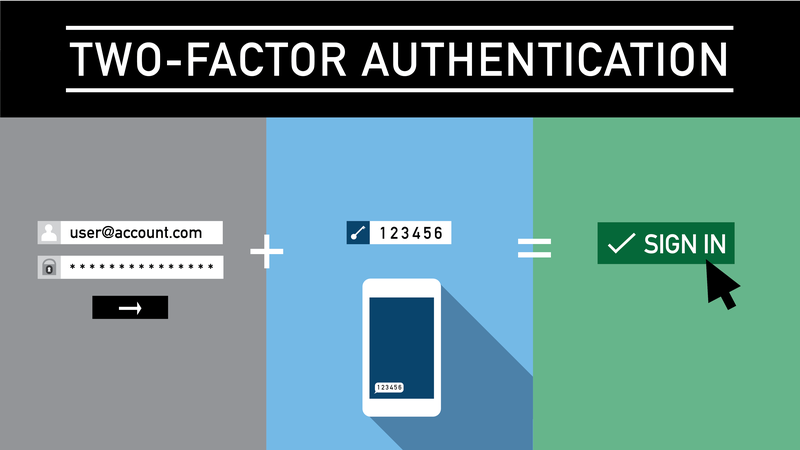
\includegraphics[width=.6\columnwidth]{img/authdouble.png}
\end{figure}}
\end{frame}




\begin{frame}
\frametitle{Tipi di account}
In base a quali operazioni ci sono consentite con il nostro account, possiamo distinguere:
\begin{itemize}
  \item \alert{account utente}, cioè un profilo personale con cui compiere operazioni di base (postare, acquistare, comunicare);\pause
  \item \alert{account amministratore}, con poteri maggiori, come cambiare impostazioni e gestire gli account utente;\pause
  \item \alert{account business}, con il potere di gestire inserzioni pubblicitarie e avere a che fare con i clienti;\pause
  \item \alert{account manager}, con il massimo dei poteri.
\end{itemize}
\end{frame}



\begin{frame}
\frametitle{Cosa sono i miei ``dati''?}
Quando parliamo dei nostri dati, questi comprendono:
\begin{itemize}
  \item nome, cognome ed eventuali altre informazioni personali;\pause
  \item le foto, i video, i messaggi che abbiamo ricevuto/inviato;\pause
  \item i file che ci riguardano (come i risultati degli esami medici);\pause
  \item i nostri username e password;\pause
  \item la cronologia delle nostre posizioni registrata dal telefono;\pause
  \item la cronologia delle pagine che abbiamo visitato;\pause
  \item il tempo passato a leggere un articolo o un post;\pause
  \item l'elenco delle nostre interazioni con altri utenti.
\end{itemize} 
\end{frame}


\begin{frame}
\frametitle{Dove sono i miei dati?}
\begin{figure}
  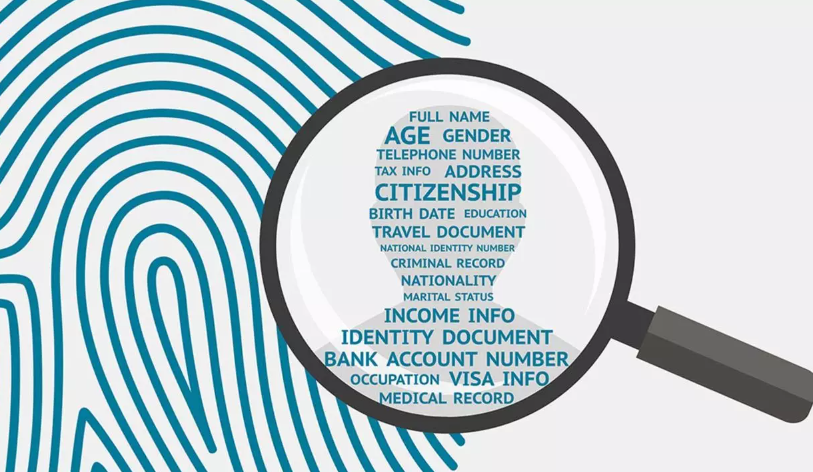
\includegraphics[width=.6\columnwidth]{img/datipers.png}
\end{figure}

I nostri dati possono essere memorizzati:

\begin{itemize}
  \item \alert{sul nostro dispositivo}, telefono o computer; in questo caso si parla di \alert{``dati locali''};\pause
  \item \alert{su un computer connesso in rete}, chiamato server; questi sono i \alert{``dati nel cloud''}.
\end{itemize}
\end{frame}


\begin{frame}
\frametitle{Cosa è il ``cloud''?}
Il cloud non è un solo oggetto, ma è una vasta \alert{rete di server collocati in tutto il mondo} che lavorano insieme.\pause

~

\begin{columns}
  \begin{column}{.5\textwidth}
    I server possono:
    \begin{itemize}
      \item archiviare e gestire dati;\pause
      \item eseguire applicazioni o distribuire contenuti o servizi:\pause
      \begin{itemize}
        \item video in streaming;\pause
        \item email;\pause
        \item software remoto;\pause
        \item social media.
      \end{itemize}
    \end{itemize}
  \end{column}
  \begin{column}{.4\textwidth}
    \begin{figure}
      
\includegraphics[width=\columnwidth]{img/cloud.jpg}
    \end{figure}
  \end{column}
\end{columns}
\end{frame}

\begin{frame}
\frametitle{Esempio: i datacenter di CloudFlare (hosting e sicurezza)}
\begin{figure}
  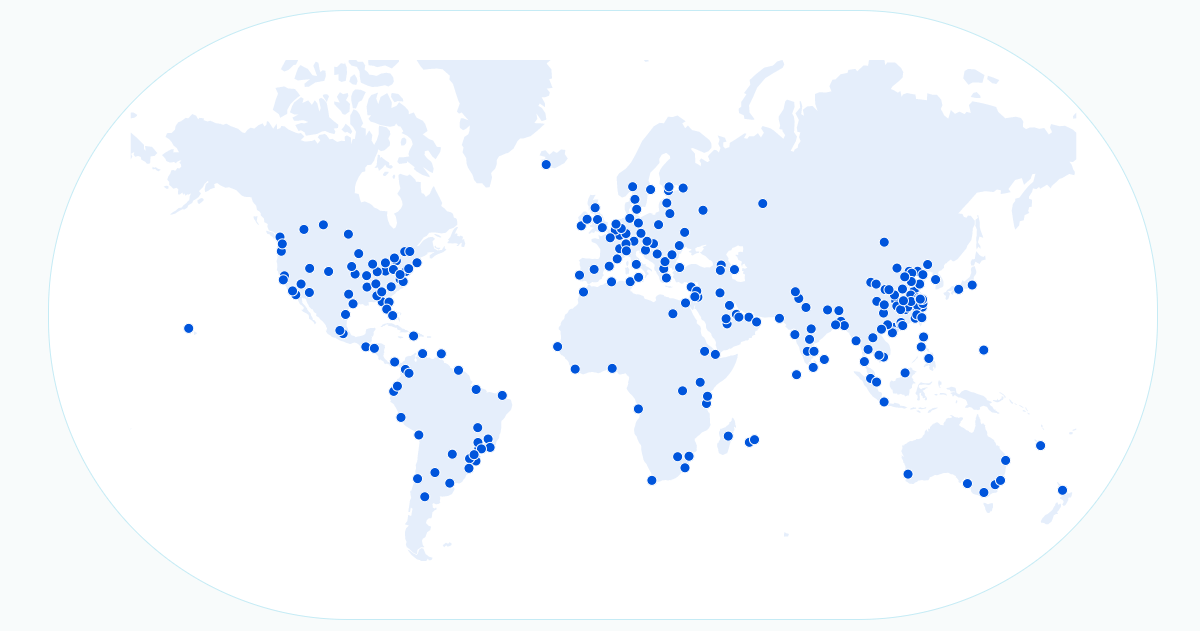
\includegraphics[width=\columnwidth]{img/cloudflarenetwork.png}
\end{figure}
\end{frame}

\section{Google}


\begin{frame}
\frametitle{Cos'è Google?}
\begin{columns}
  \begin{column}{.5\textwidth}
    Google nasce nel 1998 come \alert{motore di ricerca}, cioè un servizio per trovare pagine web a partire da parole chiave.\pause

~

Con gli anni si è sviluppata fino a trattare quasi ogni ambito del mondo informatico.\pause

~

Oggi offre email, archiviazione online, software d'ufficio online, sistemi operativi, software per la navigazione in auto e molto altro.
  \end{column}
  \begin{column}{.4\textwidth}
    \begin{figure}
      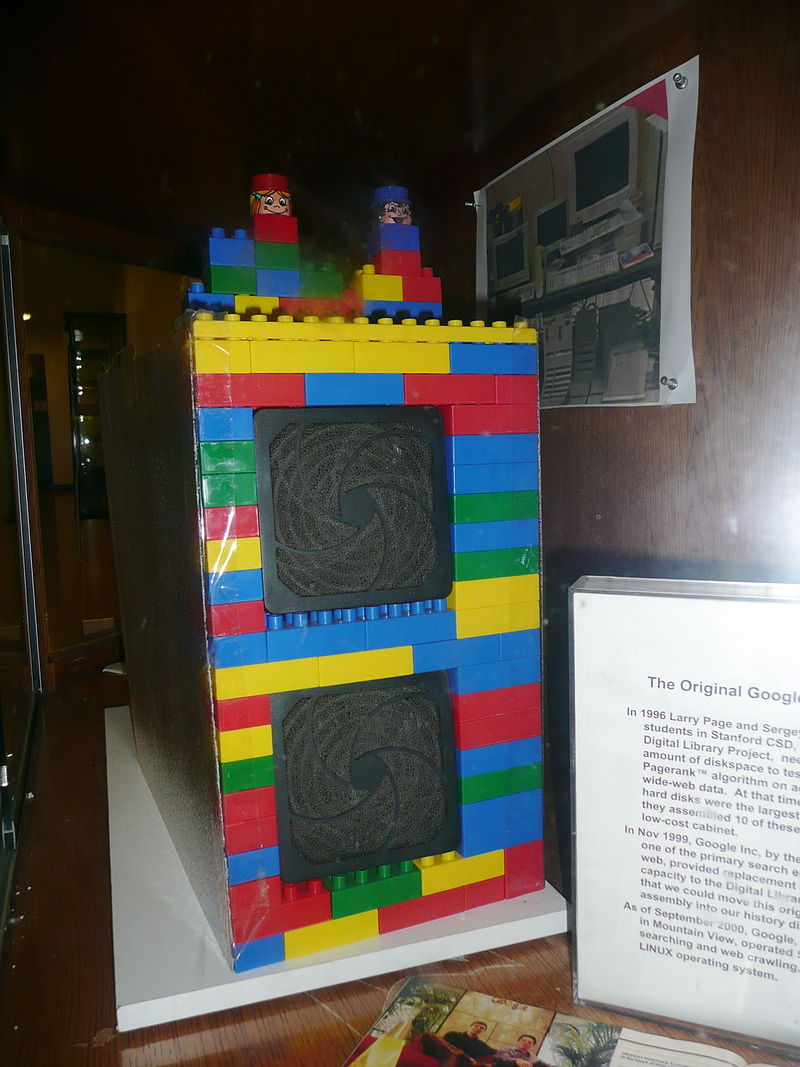
\includegraphics[width=\columnwidth]{img/servergoogle.jpg}

      Il primo server di Google
    \end{figure}
  \end{column}
  \end{columns}
\end{frame}



\begin{frame}
\frametitle{Account Google}
\begin{figure}
  
\includegraphics[width=.5\columnwidth]{img/googlesearch.png}
\end{figure}
Il \alert{motore di ricerca} di Google può essere utilizzato da tutti, mentre per gli altri servizi è necessario un \alert{account Google}.

\begin{figure}
  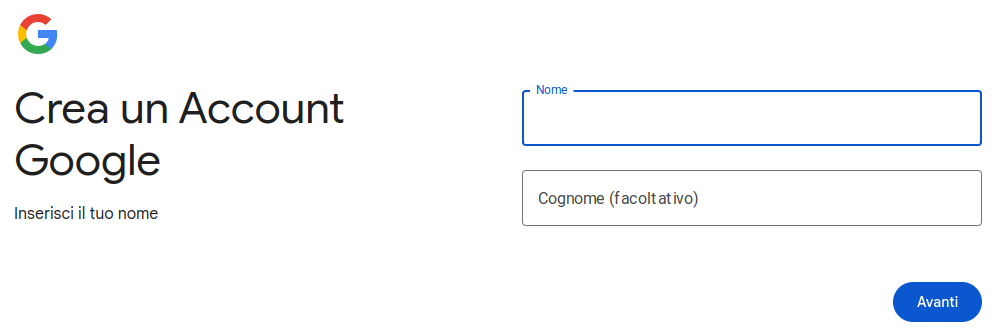
\includegraphics[width=.8\columnwidth]{img/accountgoogle.png}
\end{figure}
\end{frame}



\begin{frame}
\frametitle{Servizi offerti da Google}
Con il nostro account Google, abbiamo accesso a:
\begin{columns}
  \begin{column}{.6\textwidth}
\begin{itemize}
  \item \alert{Gmail}, servizio di posta elettronica;\pause
  \item \alert{Drive}, per salvare file nel cloud;\pause
  \item \alert{Calendar}, agenda elettronica;\pause
  \item \alert{Maps}, per strade, mappe, negozi;\pause
  \item \alert{Contatti}, per gestire i nostri numeri di telefono e indirizzi email;\pause
  \item \alert{Fogli, Documenti, Presentazioni}, una suite d'ufficio gratis online;
  \item molto altro.
\end{itemize}
  \end{column}
  \begin{column}{.3\textwidth}
    \begin{figure}
      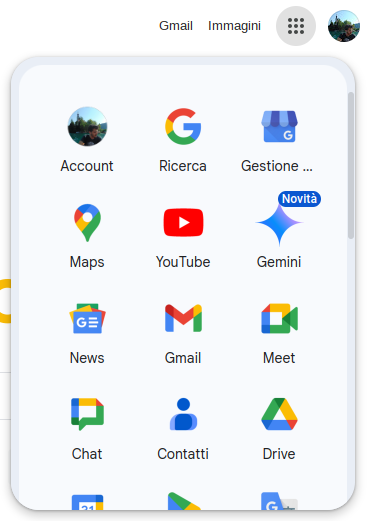
\includegraphics[width=\columnwidth]{img/googleserv.png}
    \end{figure}
  \end{column}
  \end{columns}
\end{frame}



\begin{frame}
\frametitle{Motori di ricerca}
Un motore di ricerca è un sito che permette di fornire un \alert<1>{elenco di pagine} che contengono informazioni che l'utente richiede.\pause

~

Le pagine sono selezionate tramite le \alert<2>{parole chiave} inserite dall'utente nella \alert<2>{casella di ricerca}.\pause

~

L'ordine con cui le pagine vengono visualizzate è stabilito da un algoritmo chiamato \alert<3>{ranking}.
\end{frame}



\begin{frame}
\frametitle{Ricerca avanzata}
Google, il motore di ricerca più utilizzato attualmente, contiene molte funzioni di ricerca avanzate:\pause
\begin{itemize}
  \item ricerca di stringa esatta, con \texttt{"nel mezzo del cammin"};\pause
  \item ricerca tramite \emph{wildcard}, cioè l'asterisco, con \texttt{nel * del cammin};\pause
  \item ricerca di pagine che non contengono una certa parola, con \texttt{-dante};\pause
  \item calcoli matematici e conversioni, da inserire direttamente nella barra di ricerca;\pause
  \item selezionare pagine pubblicate in date specifiche, scritte in una certa lingua, ecc.;\pause
  \item trovare immagini con specifiche caratteristiche di colore, dimensione, proporzioni, stile. 
\end{itemize}
\end{frame}


\begin{frame}
\frametitle{Esempio}
\begin{columns}
\begin{column}{.5\textwidth}
  \begin{figure}
    Ricerca:\\\texttt{Italia}

    ~

    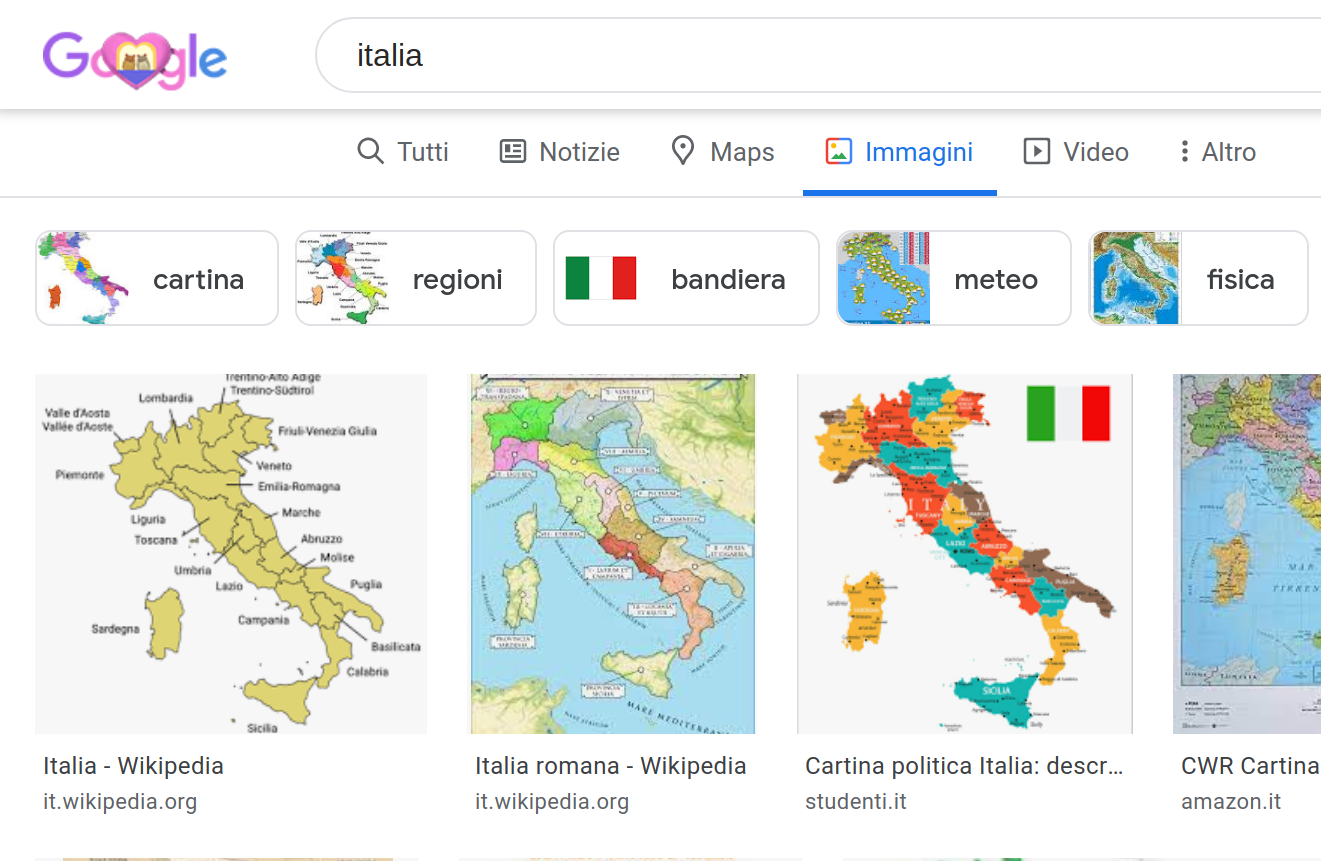
\includegraphics[width=\columnwidth]{img/italia.png}
  \end{figure}
\end{column}
\begin{column}{.5\textwidth}
  \begin{figure}
    Ricerca:\\\texttt{Italia -mappa}
    
    ~

    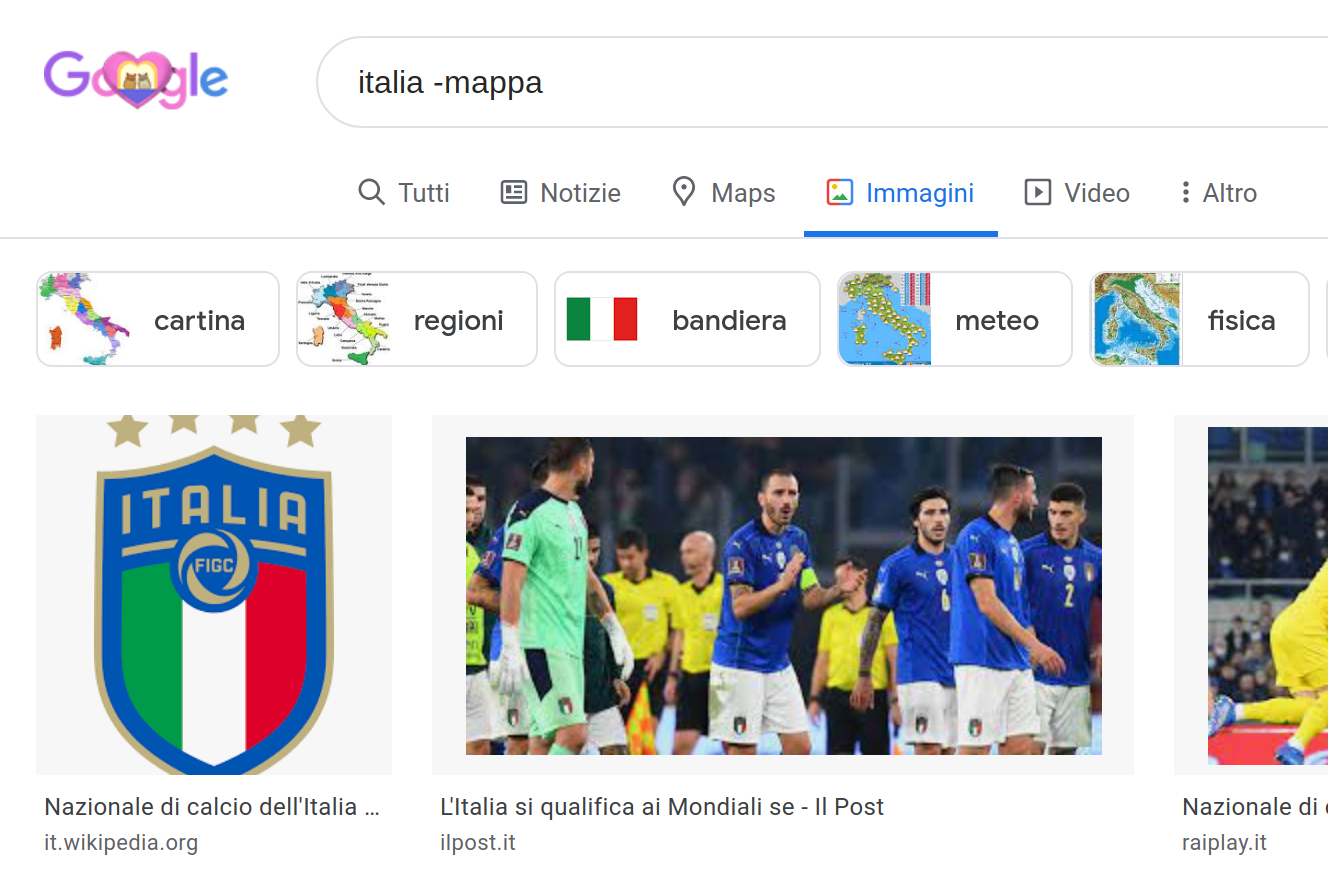
\includegraphics[width=\columnwidth]{img/italia2.png}
  \end{figure}
\end{column}
\end{columns}
\end{frame}



\section{Drive}



\begin{frame}
\frametitle{Google Drive}
La parola ``Drive'' qui non significa ``guidare'' ma ``dispositivo'', come in \emph{hard disk drive} (unità disco rigido).\pause

~

Google Drive è uno \alert{spazio di archiviazione online}: Google mette a disposizione 15 GB di spazio di archiviazione gratuito con ogni account. Le nostre mail di Gmail sono ad esempio salvate in Drive.\pause

~

Se vogliamo più spazio, dobbiamo sottoscrivere un piano a pagamento.
\end{frame}

\begin{frame}
\frametitle{Screenshot di Google Drive}
\begin{figure}
  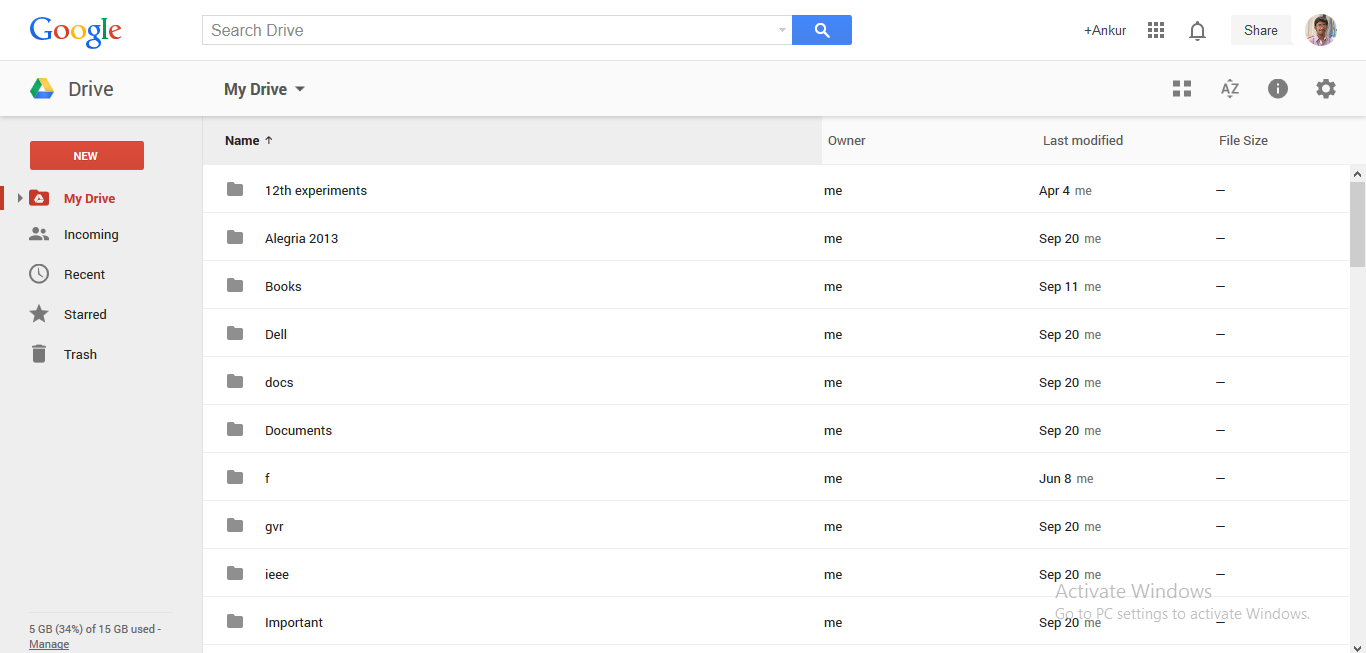
\includegraphics[width=\columnwidth]{img/drivescreen.png}
\end{figure}

La gestione dei file è molto simile a quella in locale (cioè sul nostro computer).
\end{frame}


\begin{frame}
\frametitle{Collaborare con altri}
Molto utile è la funzione di \alert{condivisione dei file}: uno stesso documento può essere visualizzato e modificato da più utenti.\pause

\begin{figure}
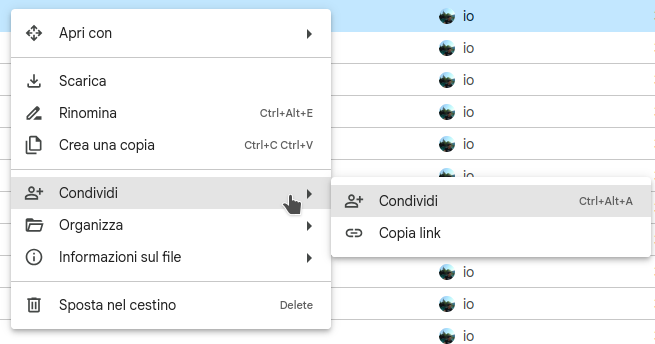
\includegraphics[width=.65\columnwidth]{img/driveshare.png}
\end{figure}

Prova a esplorare la sezione ``Condividi'' facendo clic destro su qualche file/cartella.
\end{frame}


\begin{frame}
\frametitle{Drive e backup dei file}
Una \alert{copia di backup} è una copia di sicurezza, utile ad esempio per recuperare i nostri file se li dovessimo perdere.\pause

~

Un telefono Android, ad esempio, esegue il backup delle nostre foto su Google Drive.\pause

~

Se il nostro spazio si sta esaurendo, possiamo andare a controllare come viene utilizzato e se possiamo eliminare qualche dato inutile.
\end{frame}



\begin{frame}
\frametitle{Guide online}
\begin{figure}

\includegraphics[width=.5\columnwidth]{img/ytlogo.jpg}

~

Guida base (italiano)
\href{https://www.youtube.com/watch?v=iOBp6zbghKM}{\texttt{https://www.youtube.com/watch?v=iOBp6zbghKM}}

~

Guida completa (inglese, attiva i sottotitoli in italiano)

\href{https://www.youtube.com/watch?v=jSRSgxMTU_M}{\texttt{https://www.youtube.com/watch?v=jSRSgxMTU\_M}}
\end{figure}
\end{frame}



\begin{frame}
\frametitle{Esercizi}
\begin{enumerate}
  \item Crea una cartella in Google Drive con nome ``Appunti di scuola''. Aggiungi alcune sottocartelle per le materie che studi e prova a caricare qualche file.
  \item Condividi la cartella creata nell'esercizio precedente con almeno due compagni, uno con permessi di editor e l'altro con permessi di sola visualizzazione. Controlla sui loro computer che abbiano accesso ai file che hai condiviso.
\end{enumerate}
\end{frame}



\section{Gmail}


\begin{frame}
\frametitle{La posta elettronica}
La posta elettronica (\alert<1>{email}) è la modalità di comunicazione più importante offerta da internet.\pause

~

\begin{columns}
  \begin{column}{0.55\textwidth}
  Un indirizzo email è costituito da un nome utente (\texttt{mariorossi.06}), dal simbolo $@$ (si legge ``at'') e da un dominio (\texttt{gmail.com}).\pause

   ~
   
   Ogni email possiede un \alert<3>{oggetto} (l'argomento del messaggio), un \alert<3>{testo/contenuto} ed eventualmente uno o più \alert<3>{allegati}.
  \end{column}
  \begin{column}{0.37\textwidth}
  \visible<3>{\begin{figure}
  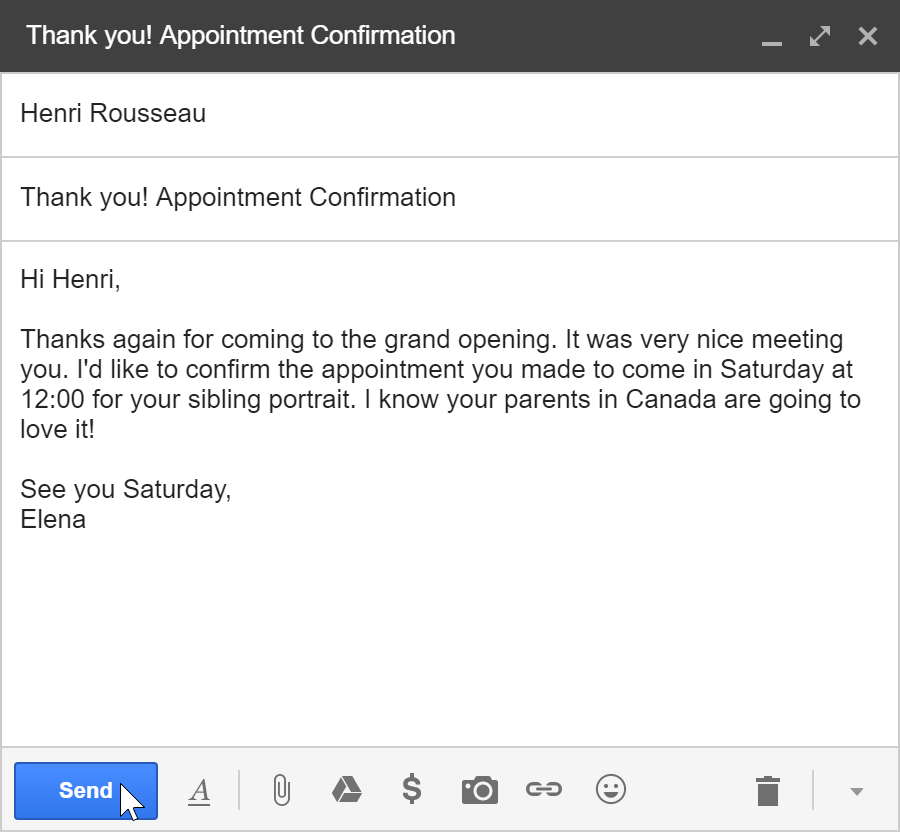
\includegraphics[width=\columnwidth]{img/email.png}
  \end{figure}}
  \end{column}
\end{columns}
\end{frame}

\begin{frame}
\frametitle{Regole d'oro per le email (1)}
\begin{enumerate}
  \item \alert{Usa un indirizzo e-mail formale.} I recapiti di posta elettronica creati da piccoli sono senz'altro simpatici, ma per dare l’immediata impressione di serietà è meglio usare un indirizzo adatto a un ambiente lavorativo. Nulla di troppo pomposo, basta servirsi del proprio nome e cognome, seguito, in caso di omonimia, dalla data di nascita: es. \texttt{ugo.rossi@email.it}.\pause
  \item \alert{L’oggetto è importante.} Chi legge la vostra email non ha tempo da perdere. Deve capire subito, leggendo l’oggetto, di cosa si parlerà e deve sentirsi invogliato ad aprirla. Pensate a qualcosa breve, ma d’effetto. Ad esempio, \emph{OGGETTO: info programma evento ``X''}.
\end{enumerate}
\end{frame}



\begin{frame}
\frametitle{Regole d'oro per le email (2)}
\begin{enumerate}\setcounter{enumi}{2}
  \item \alert{Ad ogni contesto il suo saluto.} Se state scrivendo a un potenziale datore di lavoro, a un’azienda o a un professore, esordire con ``Ciao'' o ``Caro'' non è la scelta migliore. Più adatti sono, invece, ``Egregio'' o ``Gentile'' seguiti da titolo e cognome del destinatario: es. \emph{Egregio Prof. Rossi}. Se non conoscete il nome, optate per un generico ``All’attenzione del responsabile ufficio/settore\ldots''.\pause
  \item \alert{Chi sei?} Se state scrivendo a una persona per la prima volta, è importante presentarsi subito. Dopo il saluto utilizzate le prima riga per presentarvi. Questo aiuterà chi riceve la riceve a orientarsi meglio nella lettura. Es. \emph{Sono Anna Russo, responsabile del Reparto Grafica}.
\end{enumerate}
\end{frame}




\begin{frame}
\frametitle{Regole d'oro per le email (3)}
\begin{enumerate}\setcounter{enumi}{4}
  \item \alert{Arriva dritto al punto.} Evitate giri di parole e andate dritti al punto, parlando della questione che nell’oggetto avete già accennato, senza essere ripetitivi. Es. \emph{Le scrivo per chiedere informazioni sul programma dell’evento}.\pause
  \item \alert{Ringrazia sempre.} Prima di salutare, è bene ringraziare il destinatario e fargli sapere se ci si aspetta una risposta. ``Grazie dell’attenzione'' e ``In attesa di notizie, le auguro buona giornata'' denotano cortesia e professionalità.\pause
  \item \alert{Ricorda i saluti.} Come nei saluti iniziali, anche per quelli finali bisogna tener presente chi sarà il destinatario. ``Cordiali saluti'' oppure ``Distinti saluti'' sono il giusto compromesso. E non dimenticate di firmarvi con nome e cognome.
\end{enumerate}
\end{frame}





\begin{frame}
\frametitle{Come scrivere un'email}
\begin{figure}
  
\includegraphics[width=.5\columnwidth]{img/ytlogo.jpg}
  
  ~
  
  Regole di base
  
  \href{https://www.youtube.com/watch?v=-pkeQ6hpfhA}{\texttt{https://www.youtube.com/watch?v=-pkeQ6hpfhA}}
\end{figure}
\end{frame}


\begin{frame}
\frametitle{Campi per i destinatari}
Esistono tre categorie di destinatari per un messaggio email:
\begin{columns}
  \begin{column}{0.5\textwidth}
  \begin{itemize}
   \item \alert<1>{A}, per uno o più destinatari principali;\pause
   \item \alert<2>{Cc} (copia per conoscenza), per destinatari secondari;\pause
   \item \alert<3>{Ccn} (copia conoscenza nascosta), per destinatari che però non possono sapere a quali altri indirizzi (in Cc) la mail è stata inviata.
  \end{itemize}
  \end{column}
  \begin{column}{0.4\textwidth}
  \begin{figure}
  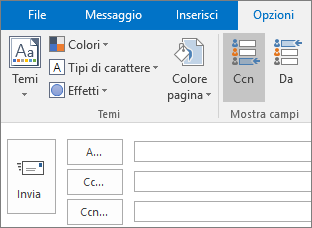
\includegraphics[width=\columnwidth]{img/accccn.png}
  \end{figure}
  \end{column}
\end{columns}
\end{frame}





\begin{frame}
\frametitle{Destinatari multipli}
Come abbiamo visto, possiamo ricevere email inviate anche ad altre persone:
\begin{figure}
  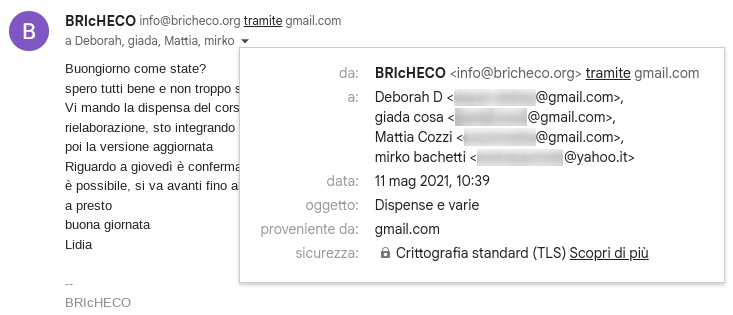
\includegraphics[width=.8\columnwidth]{img/gmaildestinatari.png}
\end{figure}\pause
In base alle esigenze, possiamo voler rispondere a tutti i destinatari oppure solo al mittente originario.
\end{frame}






\begin{frame}
\frametitle{Tipi di risposta a una mail}
\begin{figure}
  
\includegraphics[width=.7\columnwidth]{img/risposte.png}
\end{figure}

~

Abbiamo diverse opzioni:
\begin{itemize}
  \item \alert{Rispondi a tutti} per inviare una mail a tutti i destinatari dell'elenco;\pause
  \item \alert{Rispondi} per scrivere solo al mittente originario;\pause
  \item \alert{Inoltra} per ``girare'' la mail a qualche altro contatto.
\end{itemize}
\end{frame}



\begin{frame}
\frametitle{Categorie}
Gmail organizza automaticamente le nostre email in diverse categorie:
\begin{figure}
  
\includegraphics[width=\columnwidth]{img/gmailcategorie.png}
\end{figure}\pause

Se crediamo che una mail sia nella categoria sbagliata, la possiamo trascinare dove vogliamo. Gmail ``imparerà'' dalle nostre scelte.
\end{frame}



\begin{frame}
\frametitle{Tenere in ordine la posta}
Una casella di posta piena di email inutili è un problema: è come provare a lavorare con un tavolo tutto ricoperto di fogli.\pause

~

Quando non vogliamo avere un messaggio di posta in primo piano, possiamo:
\begin{itemize}
  \item \alert{eliminare il messaggio}, se siamo sicuri che non ci servirà (rimane nel cestino per 30 giorni);\pause
  \item \alert{archiviare il messaggio}, in modo che rimanga non visibile ma comunque recuperabile con una ricerca.\pause
\end{itemize}

~

L'archiviazione dei messaggi è ottima se usata insieme alle \alert{etichette} e ai \alert{filtri automatici}.
\end{frame}



\begin{frame}
\frametitle{Guida online}
\begin{figure}
  
\includegraphics[width=.5\columnwidth]{img/ytlogo.jpg}
  
  ~
  
  Utilizzo delle etichette e dei filtri
  
  \href{https://www.youtube.com/watch?v=WAIRY9dxpTk}{\texttt{https://www.youtube.com/watch?v=WAIRY9dxpTk}}
\end{figure}
\end{frame}



\begin{frame}
\frametitle{Newsletter}
Una \alert{newsletter} è un messaggio di posta inviato a molti destinatari per inviare informazioni o promozioni.\pause

~

Spesso ci iscriviamo alle newsletters quando non controlliamo bene cosa stiamo accettando quando creiamo un account.\pause

~

Chi invia newsletter, deve mettere in fondo ad ogni messaggio un \alert{link per disiscriversi}: prova a cercarlo nelle newsletters che ricevi.

\visible<3->{\begin{figure}
  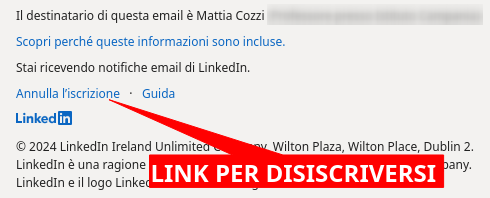
\includegraphics[width=.6\columnwidth]{img/newsletter.png}
\end{figure}}
\end{frame}



\begin{frame}
\frametitle{Esercizi}
\begin{enumerate}
  \item Crea un'etichetta ``ECFoP'' nella tua casella di posta.
  \item Imposta un filtro automatico, in modo che tutte le email contenenti la parola ``ecfop'' vengano etichettate con l'etichetta che hai creato nell'esercizio precedente.
  \item Crea un'altra etichetta ed un altro filtro automatico a tua scelta.
\end{enumerate}
\end{frame}



\section{Contatti}

\begin{frame}
\frametitle{Introduzione}
Quando abbiamo un'attività (o semplicemente vogliamo fare le cose per bene), è fondamentale avere una lista di contatti \alert{completa} e \alert{ordinata}.\pause

~

Google ci mette a disposizione una \alert{rubrica elettronica} chiamata Google Contacts.

~

\visible<2->{\begin{figure}
  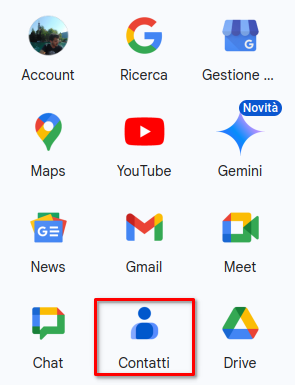
\includegraphics[width=.25\columnwidth]{img/contatti.png}
\end{figure}}
\end{frame}



\begin{frame}
\frametitle{Schermata principale}
\begin{figure}
  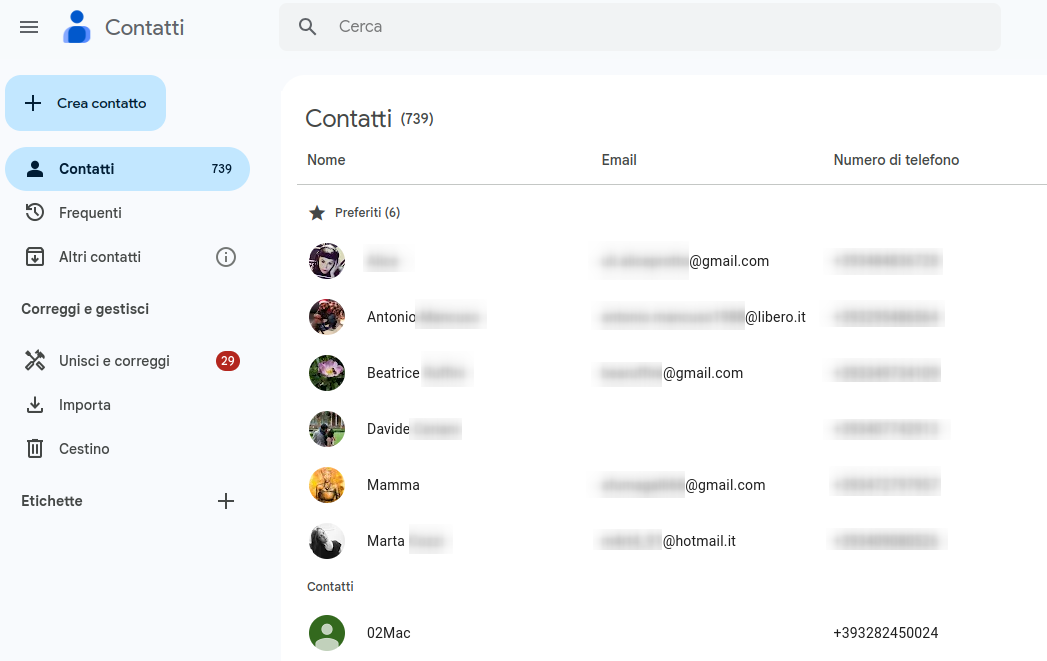
\includegraphics[width=\columnwidth]{img/contatti2.png}
\end{figure}
\end{frame}




\begin{frame}
\frametitle{Aggiungere un contatto da Gmail}
Possiamo aggiungere facilmente un contatto da Gmail passando con il mouse sopra all'indirizzo che vogliamo aggiungere alla nostra rubrica.

\begin{figure}
  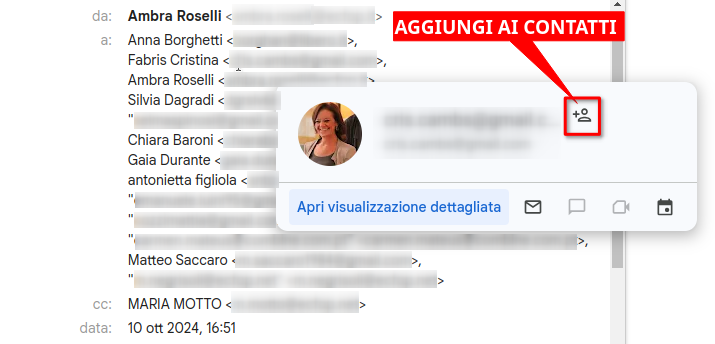
\includegraphics[width=.8\columnwidth]{img/aggiungicontatto.png}
\end{figure}
\end{frame}





\begin{frame}
\frametitle{Creazione e modifica contatto}
\begin{columns}
  \begin{column}{.4\textwidth}
    Dalla schermata principale, clicchiamo su ``Crea contatto'' e scegliamo di crearne uno solo.\pause

    ~
    
    Possiamo aggiungere molte informazioni, molto utile se stiamo creando una \alert{rubrica lavorativa}.\pause

    ~

    Per modificare un contatto, usiamo l'icona della matita dall'elenco principale.
  \end{column}
  \begin{column}{.5\textwidth}
    \begin{figure}
      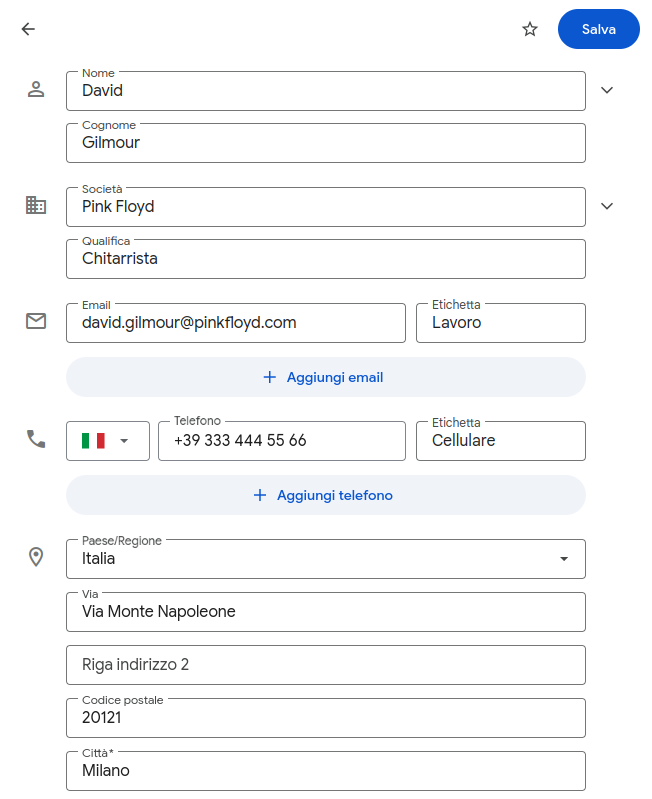
\includegraphics[width=\columnwidth]{img/nuovocontatto.png}
    \end{figure}
  \end{column}
\end{columns}
\end{frame}


\begin{frame}
\frametitle{Etichette}
Possiamo raggruppare i contatti con le etichette.\pause

~

Cercando poi i contatti nella nostra rubrica li possiamo etichettare.

\visible<2->{\begin{figure}
  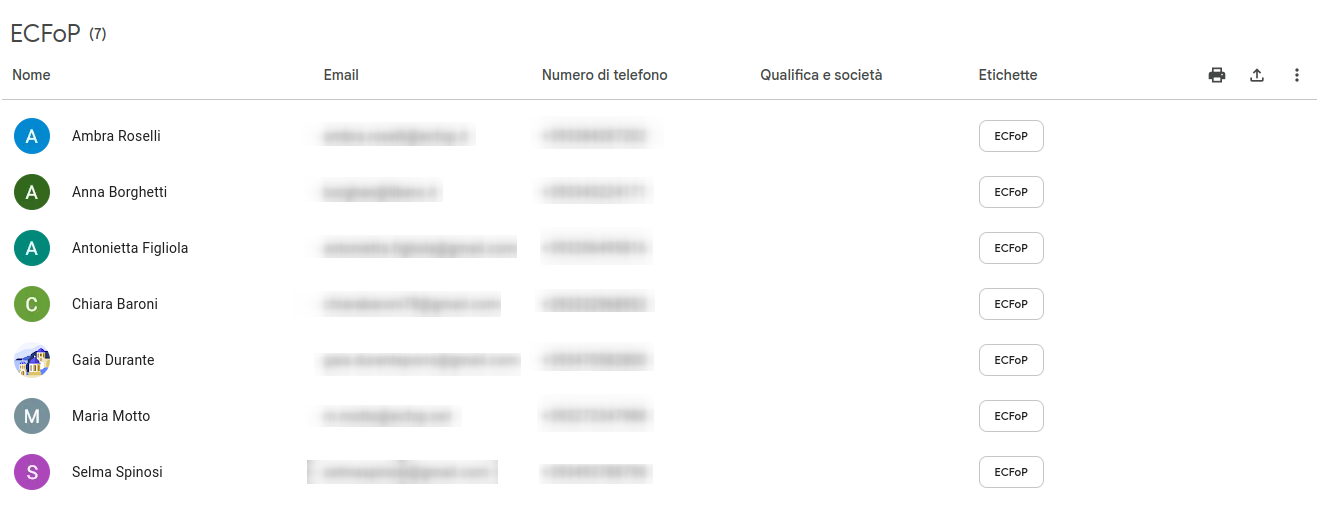
\includegraphics[width=.9\columnwidth]{img/etichettecontatti.png}
\end{figure}}
\end{frame}



\begin{frame}
\frametitle{Esportare contatti}
Selezionando un gruppo di contatti (o un'etichetta), dal menu con i tre puntini possiamo esportare i dati, cioè \alert{scaricare un file} che contiene tutti i contatti selezionati, con i dettagli in un ordine ben preciso.\pause

~

Il formato più semplice è \alert{CSV Outlook}, che possiamo aprire con Excel.
\visible<2->{\begin{figure}
  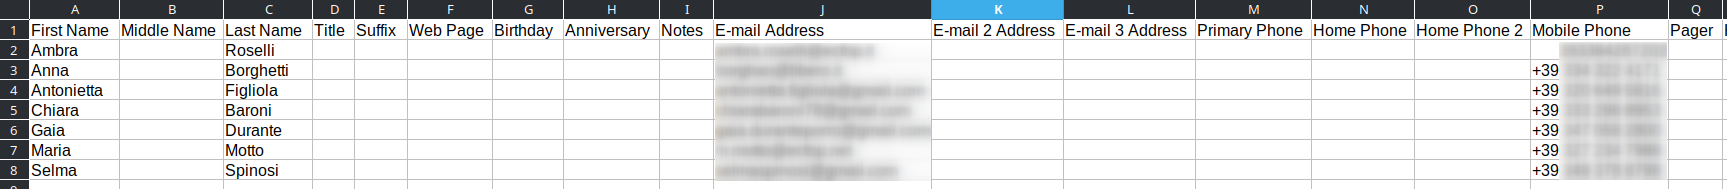
\includegraphics[width=\columnwidth]{img/csv.png}
\end{figure}}\pause

~

Molto utile se dobbiamo inviare molti contatti a qualcuno!
\end{frame}




\begin{frame}
\frametitle{Importare contatti}
Importare è l'opposto di esportare: possiamo caricare velocemente un gran numero di contatti mediante un \alert{file sul nostro computer}.\pause

~

Partiamo da un file CSV Outlook, come quello precedente, e clicchiamo su ``Importa'' dalla schermata principale.

\visible<2->{\begin{figure}
  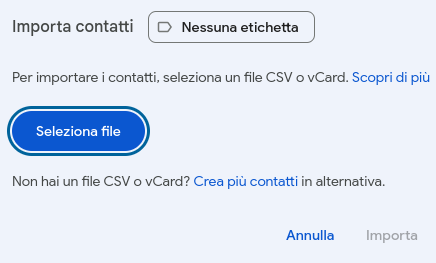
\includegraphics[width=.5\columnwidth]{img/importacontatti.png}
\end{figure}}
\end{frame}




\begin{frame}
\frametitle{Guida online}
\begin{figure}

\includegraphics[width=.5\columnwidth]{img/ytlogo.jpg}

~

Guida completa (inglese, attiva i sottotitoli in italiano)

\href{https://www.youtube.com/watch?v=NW3dDdbgLLA}{\texttt{https://www.youtube.com/watch?v=NW3dDdbgLLA}}
\end{figure}
\end{frame}




\begin{frame}
\frametitle{Esercizi}
\begin{enumerate}
  \item Aggiungi ai contatti di Google l'indirizzo mail (e se vuoi anche il numero di telefono) di tutti i tuoi compagni di classe.
  \item Crea un gruppo di contatti etichettati con la tua classe, come ad esempio ``3a PAN''.
  \item Esporta tutti i contatti del gruppo precedente in formato CSV Outlook.
\end{enumerate}
\end{frame}





\begin{frame}
\frametitle{Esercizi}
\begin{enumerate}\setcounter{enumi}{3}
  \item Utilizzando come base il file che hai scaricato nell'esercizio precedente, crea con Excel un nuovo file CSV con i contatti mostrati in tabella e importalo in Contacts.
\end{enumerate}
\begin{table}[]\def\arraystretch{1.5}\footnotesize
  \begin{tabular}{|l|l|l|l|}\hline
  \textbf{Nome} & \textbf{Cognome} & \textbf{Email}               & \textbf{Telefono} \\\hline
  Nick          & Mason            & \texttt{nick.mason@pinkfloyd.com}     & +39 333 111 22 33 \\\hline
  Roger         & Waters           & \texttt{roger.waters@pinkfloyd.com}   & +39 333 222 33 44 \\\hline
  Richard       & Wright           & \texttt{richard.wright@pinkfloyd.com} & +39 333 333 44 55 \\\hline
  David         & Gilmour          & \texttt{david.gilmour@pinkfloyd.com}  & +39 333 444 55 66 \\\hline
  \end{tabular}
\end{table}
\end{frame}


\section{Calendar}

\begin{frame}
\frametitle{Cos'è Google Calendar}
Google Calendar è l'\alert{agenda elettronica} della suite Google.\pause

~

\begin{columns}
\begin{column}{.7\textwidth}
  Permette di:
  \begin{itemize}
    \item gestire i propri appuntamenti;\pause
    \item gestire gli appuntamenti di un gruppo di persone;\pause
    \item programmare eventi ricorrenti;\pause
    \item programmare videochiamate;\pause
    \item creare eventi a cui invitare partecipanti esterni.
  \end{itemize}  
\end{column}
\begin{column}{.2\textwidth}
  \begin{figure}
    
\includegraphics[width=\columnwidth]{img/calendarlogo.png}
  \end{figure}
\end{column}
\end{columns}
\end{frame}


\begin{frame}
\frametitle{Interfaccia principale}
\begin{figure}
  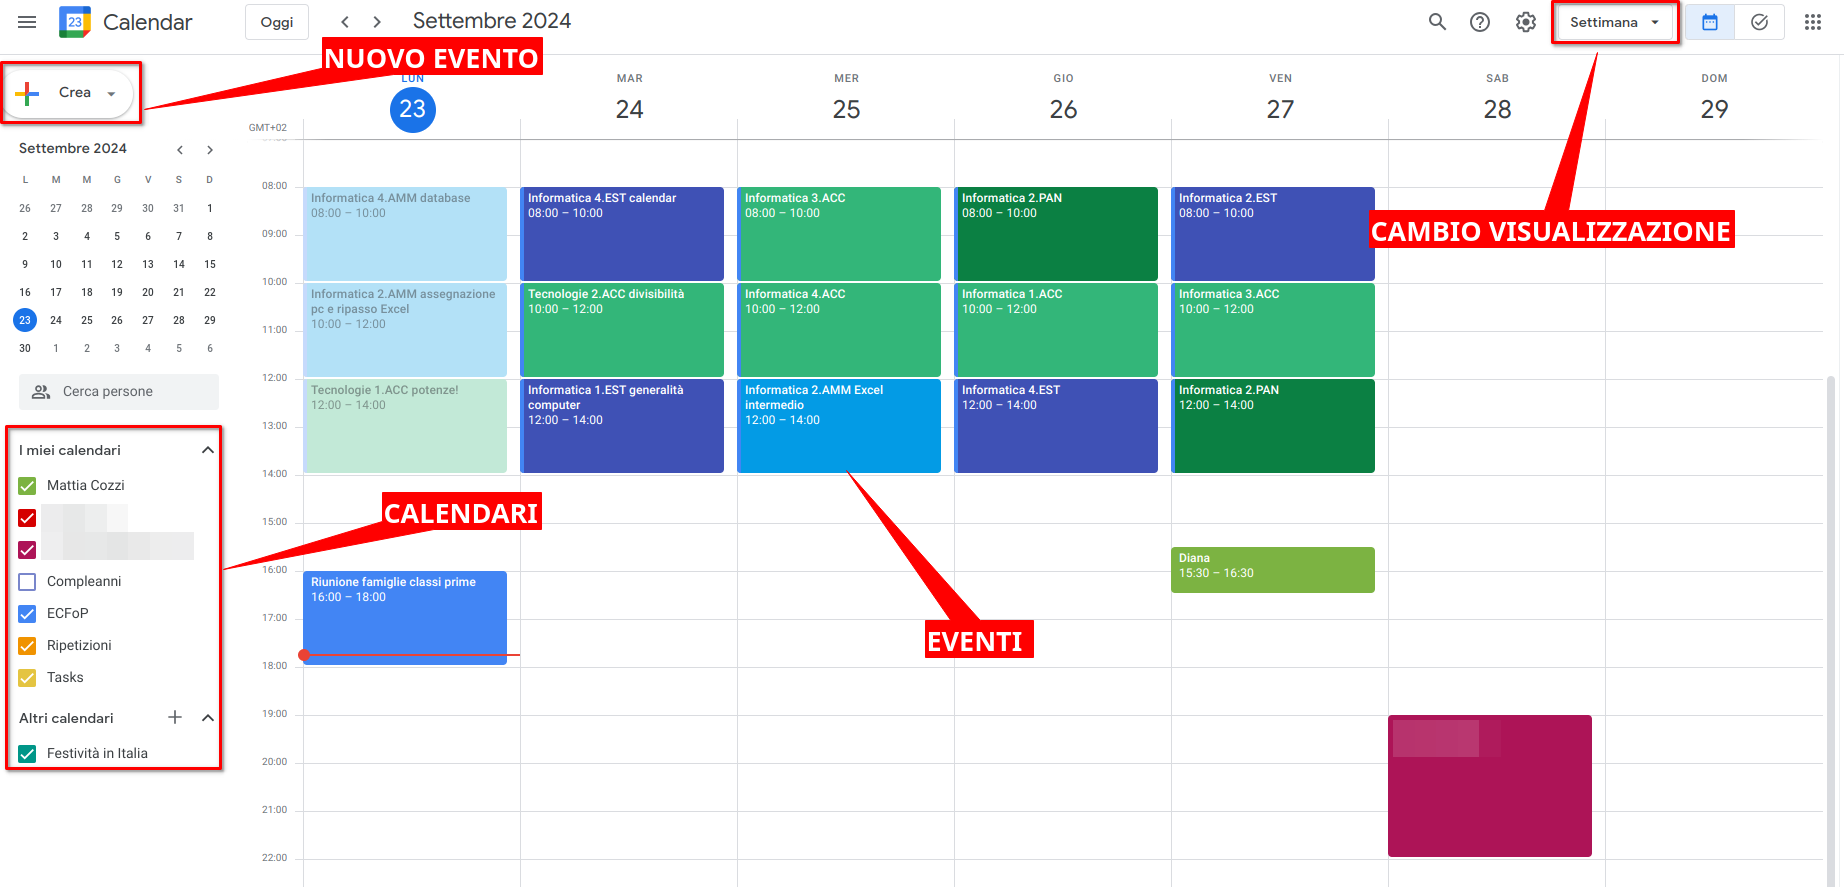
\includegraphics[width=\columnwidth]{img/calendar1.png}
\end{figure}
\end{frame}

\begin{frame}
\frametitle{Opzioni di visualizzazione}
\begin{figure}
  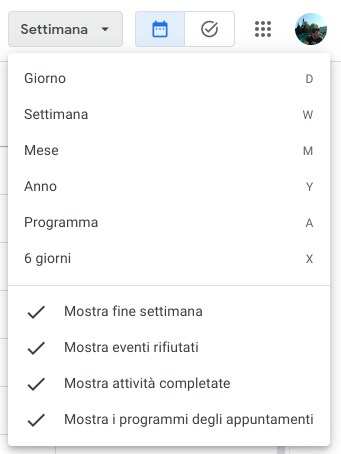
\includegraphics[width=.35\columnwidth]{img/calendarvisua.png}
\end{figure}

~

È possibile cambiare la porzione di tempo visualizzata.\pause

~

Attenzione alle scorciatoie!
\end{frame}


\begin{frame}
\frametitle{Creazione di un evento}
\begin{figure}
  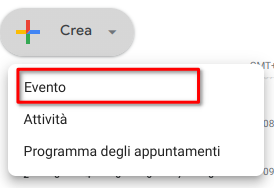
\includegraphics[width=.3\columnwidth]{img/calendarcrea.png}
\end{figure}
Apriamo la \alert{finestra rapida} di creazione evento.
\end{frame}



\begin{frame}
\frametitle{Finestra rapida creazione evento}
Questa finestra contiene alcune opzioni per la creazione di un nuovo evento, ma non tutte.

\begin{figure}
  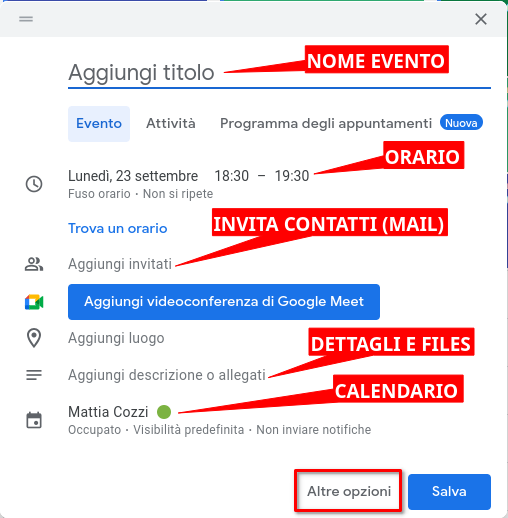
\includegraphics[width=.5\columnwidth]{img/calendarcrea2.png}
\end{figure}
\end{frame}

\begin{frame}
\frametitle{Invitati}
Scrivendo degli indirizzi email nello spazio per gli invitati, si condivide l'evento che stiamo creando con qualcuno.

~

Gli invitati ricevono una mail di invito, da cui possono decidere se accettare o meno. Se accettano, vedranno l'evento nel proprio calendario.

~

Quando si invita qualcuno, Calendar aggiunge automaticamente l'opzione per una videochiamata tramite Google Meet.
\end{frame}


\begin{frame}
\frametitle{Descrizione}
Molto utile la descrizione dell'evento, che può essere usata per:
\begin{columns}
  \begin{column}{.5\textwidth}
\begin{itemize}
  \item appunti;
  \item ordini del giorno di una riunione;
  \item file utili (posso allegare ricette mediche ad un appuntamento col dottore);
  \item commenti degli utenti coinvolti nell'evento.
\end{itemize}
  \end{column}
  \begin{column}{.4\textwidth}
    \begin{figure}
      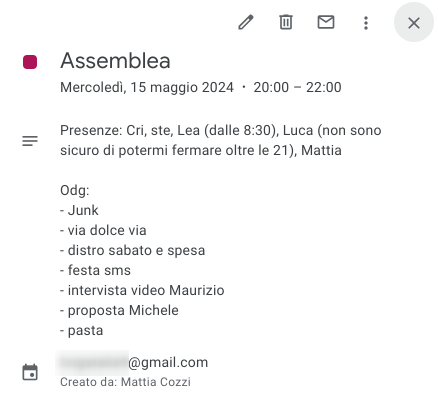
\includegraphics[width=\columnwidth]{img/calendarnotes.png}
    \end{figure}
  \end{column}
\end{columns}

\end{frame}


\begin{frame}
\frametitle{Modifica di un evento}
Una volta creato un evento, possiamo cambiarne il colore o eliminarlo facendo destro clic sull'evento.

\begin{figure}
  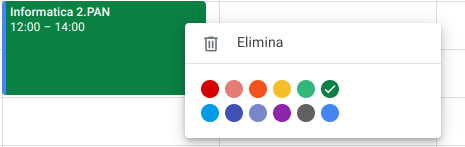
\includegraphics[width=.6\columnwidth]{img/calendarcolore.png}
\end{figure}

Trascinando i bordi di un evento possiamo inoltre modificarne graficamente la durata.

~

Trascinando l'evento posso spostarlo nel tempo.
\end{frame}



\begin{frame}
\frametitle{Più calendari}
Google Calendar può gestire diversi calendari contemporaneamente.

~

\begin{columns}
  \begin{column}{.5\textwidth}
    Organizzare il proprio lavoro con diversi calendari è utile per:
\begin{itemize}
  \item separare diverse attività: lavoro, studio, tempo libero;\pause
  \item gestire il calendario di più dipendenti/collaboratori;\pause
  \item condividere eventi con amici e parenti.
\end{itemize}
  \end{column}
  \begin{column}{.4\textwidth}
    \begin{figure}
      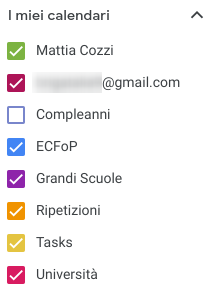
\includegraphics[width=\columnwidth]{img/calendarcals.png}
    \end{figure}
  \end{column}
\end{columns}
\end{frame}


\begin{frame}
\frametitle{Creazione di un calendario}
\begin{figure}
  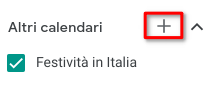
\includegraphics[width=.2\columnwidth]{img/calendarnuovocal.png}
\end{figure}
Per creare un nuovo calendario, clicchiamo sul + vicino ad ``Altri calendari''.

\begin{figure}
  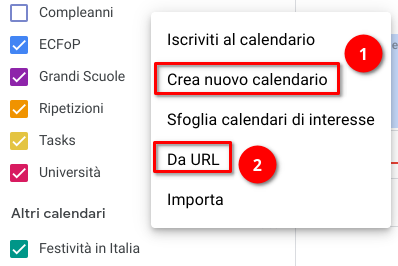
\includegraphics[width=.4\columnwidth]{img/calendarnuovocal2.png}
\end{figure}
L'opzione ``Da URL'' permette di iscriversi ad un calendario a cui siamo stati invitati tramite link (URL è sinonimo di link).
\end{frame}


\begin{frame}
\frametitle{Opzioni calendario}
Una volta creato un calendario, possiamo modificarne le proprietà cliccando sui tre puntini a fianco al nuovo calendario nell'interfaccia principale.

\begin{figure}
  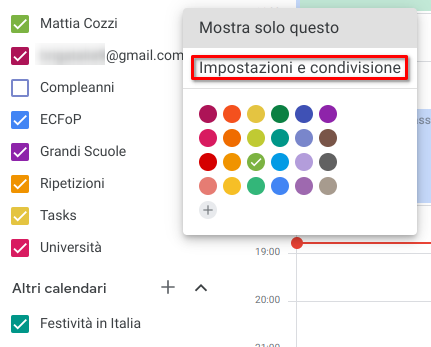
\includegraphics[width=.5\columnwidth]{img/calendarcalmod.png}
\end{figure}
\end{frame}



\begin{frame}
\frametitle{Condivisione di un calendario}
Dalla finestra delle opzioni calendario:
\begin{figure}
  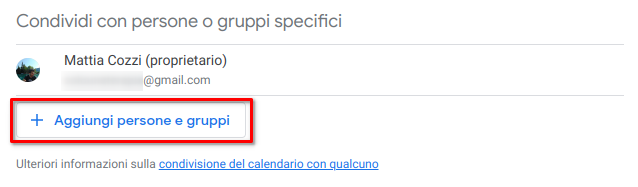
\includegraphics[width=.5\columnwidth]{img/calendarshare.png}
\end{figure}

\begin{columns}
  \begin{column}{.5\textwidth}
    \begin{figure}
      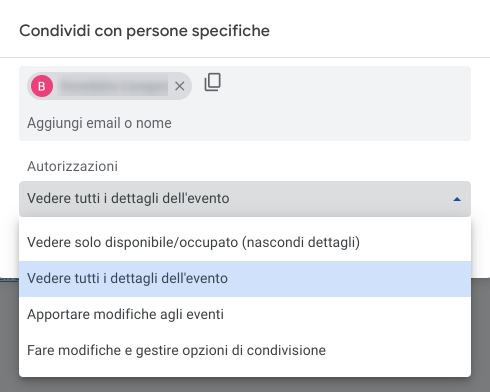
\includegraphics[width=\columnwidth]{img/calendarshare2.png}
    \end{figure}
  \end{column}
  \begin{column}{.4\textwidth}
    Un invitato può avere permessi (cioè ``poteri'') diversi.

    ~

    Gli invitati ricevono una mail, da cui possono decidere se accettare l'invito. Se sì, vedranno il nuovo calendario insieme ai loro.
  \end{column}
\end{columns}
\end{frame}

\begin{frame}
\frametitle{Finestra completa creazione evento}
La apriamo cliccando su ``Altre opzioni'' nella finestra rapida di creazione evento.

\begin{figure}
  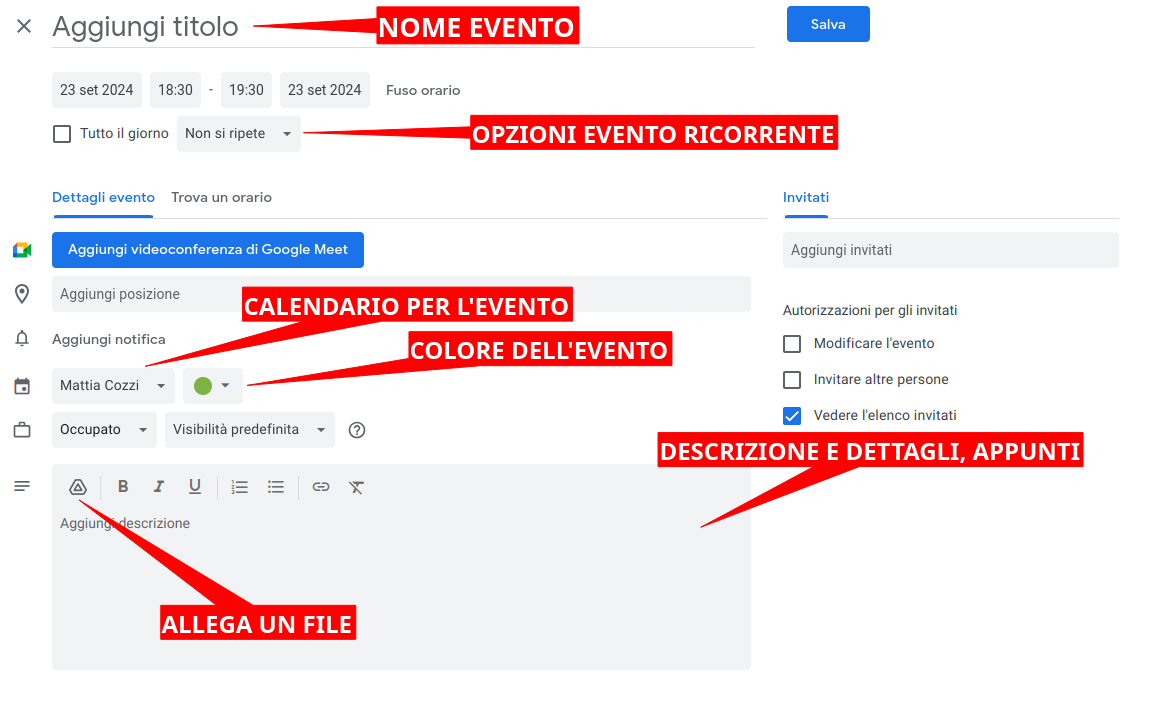
\includegraphics[width=\columnwidth]{img/calendarevento.png}
\end{figure}
\end{frame}

\begin{frame}
\frametitle{Eventi ricorrenti}
Spesso un evento si ripete nel tempo, come ad esempio:
\begin{itemize}
  \item un orario scolastico \begin{center}``tutti i lunedì alle 11 c'è matematica''\end{center}\pause
  \item un cliente ricorrente \begin{center}``la signora Rossi viene tutti i venerdì alle 10.30''\end{center}\pause
  \item un'attività ripetitiva \begin{center}``bagnare le piante ogni 10 giorni''\end{center}\pause
  \item un corso di qualche tipo \begin{center}``il corso di ceramica è  formato da 10 incontri tutti i lunedì sera, a partire dal 23 settembre''\end{center}\pause
\end{itemize}

~

Calendar contiene utilissime funzioni per gestire gli eventi ricorrenti.
\end{frame}

\begin{frame}
\frametitle{Impostazione eventi ricorrenti}
Possiamo impostare la ripetizione di un evento dalla pagina (anche rapida) di modifica evento:
\begin{figure}
  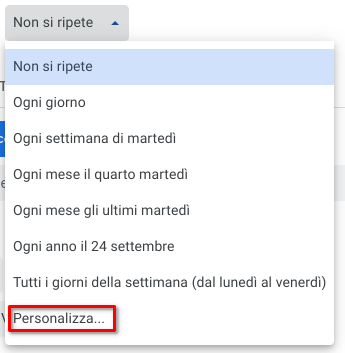
\includegraphics[width=.4\columnwidth]{img/calendarricorrente.png}
\end{figure}
Le opzioni più interessanti si trovano su ``Personalizza''.
\end{frame}




\begin{frame}
\frametitle{Guide online}
\begin{figure}

\includegraphics[width=.5\columnwidth]{img/ytlogo.jpg}

~

Guida 1 (italiano)

\href{https://www.youtube.com/watch?v=eIbLRVJj8Mw}{\texttt{https://www.youtube.com/watch?v=eIbLRVJj8Mw}}

~

Guida 2 (inglese, attiva i sottotitoli in italiano)

\href{https://www.youtube.com/watch?v=XNGqA6I1b24}{\texttt{https://www.youtube.com/watch?v=XNGqA6I1b24}}
\end{figure}
\end{frame}



\begin{frame}
\frametitle{Esercizi}
\begin{enumerate}
  \item Crea un'agenda per la gestione di uno studio estetico o di acconciatura con le seguenti caratteristiche:
  \begin{itemize}
    \item tre calendari diversi (con anche colori diversi) per tre diversi collaboratori/collaboratrici dello studio;
    \item se riesci, invita dei tuoi compagni a partecipare come collaboratori (avrai bisogno dei loro indirizzi email);
    \item una settimana di appuntamenti piena, per tutti e tre collaboratori, dalle 9.00 alle 17.00;
    \item appuntamenti della durata da un'ora a due ore;
    \item pausa pranzo dalle 13.00 alle 14.00 (lasciare senza eventi).
  \end{itemize}
\end{enumerate}
\end{frame}

\begin{frame}
  \frametitle{Esercizi}
  \begin{enumerate}\setcounter{enumi}{1}
    \item Completa l'agenda precedente aggiungendo:
    \begin{itemize}
      \item una breve descrizione per ogni evento;
      \item un allegato (PDF o immagine) per ogni evento del martedì;
      \item ripetizione per 10 volte per almeno 5 appuntamenti.
      \item ripetizione fino a fine giugno per almeno 3 appuntamenti.
    \end{itemize}
  \end{enumerate}
\end{frame}

\begin{frame}
  \frametitle{Esercizi}
  \begin{enumerate}\setcounter{enumi}{2}
    \item Aggiungi all'agenda creata in precedenza gli eventi che puoi dedurre dalle seguenti email ricevute (sostituisci XXX e YYY con quello che ritieni più opportuno).
    
    ~

    \begin{itemize}
      \item Buongiorno, vorrei prenotare un trattamento XXX con la vostra estetista/parrucchiera YYY per venerdì prossimo. Io posso arrivare per le 11.00, in un'ora circa dovrei aver finito.

      Grazie e buona giornata, Anna

      ~
      \item Ciao a tutte, confermo la mia disponibilità a collaborare con il vostro studio tutti i martedì e i venerdì mattina, dalle 9.00 fino alla pausa pranzo. Potete iniziare a considerarmi nella vostra programmazione. Posso iniziare già la prossima settimana, e sarò disponibile a collaborare con voi fino alla metà di luglio.

      Attenzione: sarò assente dal lavoro il primo martedì di maggio e l'ultimo venerdì di giugno, per via di impegni personali.

      Ciao e a presto, Valentina
    \end{itemize}
  \end{enumerate}
\end{frame}



\section{Moduli}

\begin{frame}
\frametitle{Introduzione}
Un modulo (o form) è un \alert{modello da compilare con dei dati}, come quelli che compiliamo a mano.

~

\begin{columns}
  \begin{column}{.5\textwidth}
    \begin{figure}
      
\includegraphics[width=\columnwidth]{img/compilazionemodulo.jpg}
    \end{figure}
  \end{column}
  \begin{column}{.3\textwidth}
    \begin{figure}
      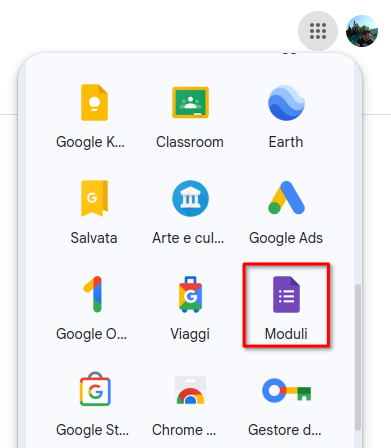
\includegraphics[width=\columnwidth]{img/moduli.png}
    \end{figure}
  \end{column}
\end{columns}\pause

~


~

\alert{Google Forms} ci permette di crearne di molto potenti, utili a raccogliere dati e files da molti utenti.
\end{frame}


\begin{frame}
\frametitle{Esempi di utilizzo}
\begin{columns}
  \begin{column}{.4\textwidth}
    \begin{figure}
      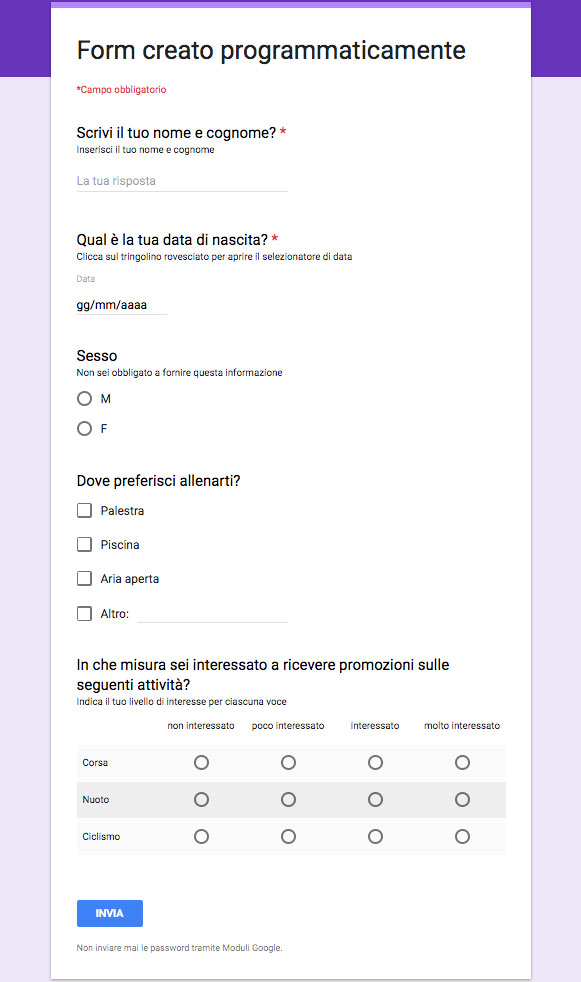
\includegraphics[width=\columnwidth]{img/form1.jpg}
    \end{figure}
  \end{column}
  \begin{column}{.6\textwidth}
\begin{itemize}
  \item Raccogliere le iscrizioni ad un corso;\pause
  \item raccogliere le prenotazioni per un evento;\pause
  \item prendere appuntamenti;\pause
  \item raccogliere dati anagrafici;\pause
  \item farsi inviare dei files;\pause
  \item creare un questionario soddisfazione clienti.
\end{itemize}
  \end{column}
\end{columns}
\end{frame}




\begin{frame}
\frametitle{Creazione di un form}
\begin{figure}
  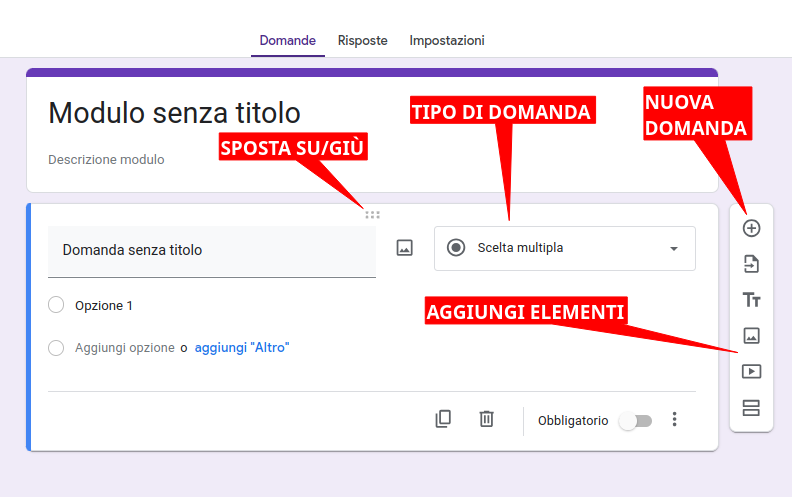
\includegraphics[width=\columnwidth]{img/form2.png}
\end{figure}
\end{frame}



\begin{frame}
\frametitle{Campi di un form}
\begin{columns}
  \begin{column}{.3\textwidth}
    \begin{figure}
      \includegraphics[width=\columnwidth]{img/form3.png}
    \end{figure}
  \end{column}
  \begin{column}{.65\textwidth}
    Ci sono diversi tipi di domande e risposte che possiamo creare.\pause

    ~

    Prova a sperimentare con le possibilità (le icone sono molto chiare).\pause

    ~

    È possibile anche far caricare agli utenti un file su Drive.
  \visible<3>{\begin{figure}
      \includegraphics[width=\columnwidth]{img/form4.png}
    \end{figure}}
  \end{column}
\end{columns}
\end{frame}


\begin{frame}
\frametitle{Creazione di un quiz}
\begin{figure}
  \includegraphics[width=.5\columnwidth]{img/form7.png}
\end{figure}
Se impostiamo il form come quiz dovremo aggiungere le ``chiavi di risposta'' (cioè le risposte corrette).
\end{frame}







\begin{frame}
\frametitle{Inviare un form}
Per inviare un form, clicchiamo sul pulsante in alto a destra.
\begin{figure}
  \includegraphics[width=.5\columnwidth]{img/form5.png}
\end{figure}
\end{frame}






\begin{frame}
\frametitle{Visualizzare le informazioni ricevute}
Nella pagina di modifica del form, clicchiamo su ``Risposte''.

\begin{figure}
  \includegraphics[width=.6\columnwidth]{img/form6.png}
\end{figure}\pause

~

Possiamo visualizzare le risposte in modi diversi, dai grafici fino alle risposte complete di tutti quelli che hanno compilato il form.
\end{frame}




\begin{frame}
\frametitle{Guide online}
\begin{figure}
\includegraphics[width=.5\columnwidth]{img/ytlogo.jpg}

~

Guida completa (italiano)

\href{https://www.youtube.com/watch?v=q1SScR0zwFc}{\texttt{https://www.youtube.com/watch?v=q1SScR0zwFc}}
\end{figure}
\end{frame}



\begin{frame}
\frametitle{Esercizi}
\begin{enumerate}
  \item Crea un modulo per l'iscrizione ad un evento a tua scelta per cui serve la prenotazione. Dovrai richiedere:
  \begin{itemize}
    \item Nome e cognome
    \item Data di nascita
    \item Numero di telefono
    \item Numeri di posti da prenotare
    \item Data per cui si vuole prenotare
    \item Consenso al trattamento dei dati personali
  \end{itemize}
  \item Invia il form che hai creato nell'esercizio precedente ad almeno 5 tuoi compagni di classe e verifica le loro risposte.
\end{enumerate}
\end{frame}






\begin{frame}
\frametitle{Esercizi}
\begin{enumerate}\setcounter{enumi}{2}
  \item Crea un modulo che raccoglie il grado di soddisfazione dei clienti di un negozio a tua scelta. Dovrai richiedere:
  \begin{itemize}
    \item Nome
    \item Negozio frequentato (con almeno tre caselle di controllo)
    \item Numeri di articoli acquistati
    \item Grado di soddisfazione da 1 (scarso) a 5 (ottimo)
    \item Ulteriori suggerimenti (opzionale, con un breve testo)
  \end{itemize}
  \item Invia il form che hai creato nell'esercizio precedente ad almeno 5 tuoi compagni di classe e verifica le loro risposte.
  \item Crea una verifica su un argomento a tua scelta, come almeno 7 domande a risposta multipla.
\end{enumerate}
\end{frame}




\end{document}
